\chapter*{Metodología}
Con el objetivo de desarrollar una plataforma que se ajuste al modelo de negocio  planteado por Ruta N, se asistió a unas sesiones de acompañamiento con el  laboratorio de creación que dispone la corporación; En estas sesiones se buscaba  plantear de manera clara la necesidad que busca solventar la plataforma, identificar el mercado objetivo y sus competencias, prototipado de la solución y por ultimo  aterrizar un modelo de negocio viable. \\

Las sesiones del laboratorio se distribuyeron en una sesión de 4 horas
semanal  durante cuatro semanas donde se utilizó una  metodología compuesta por conceptos  de design thinking (ver figura 1) y  metodología doble diamante (ver figura 2).


\begin{figure}[ht]
  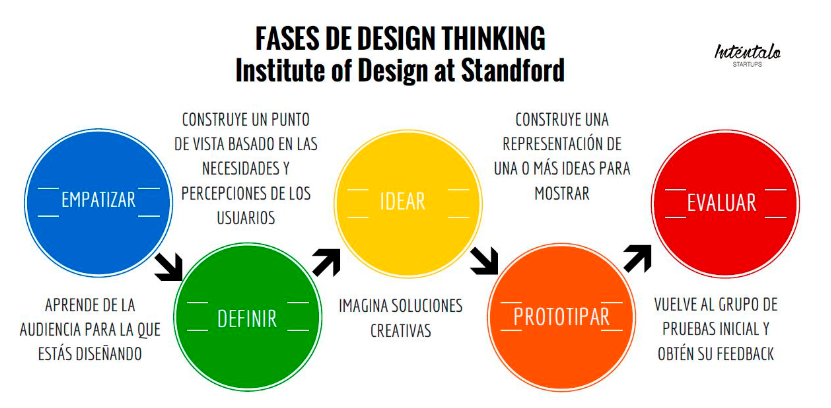
\includegraphics[width=\linewidth, center]{images/design_thinking.PNG}
  \caption{Proceso de la metodologia Design thinking. Tomado de \url{http://cursoparaemprendedoresuned.intentalo.es}}
  \label{fig:img1}
\end{figure}

\begin{figure}[ht]
  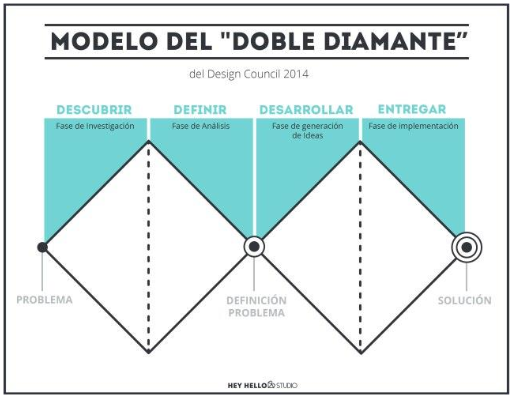
\includegraphics[scale=0.8, center]{images/doble_diamante.PNG}
  \caption{Proceso de la metodologia Doble diamante. Tomado de \url{https://i.pinimg.com}}
  \label{fig:img2}
\end{figure}


\begin{itemize}
    \item Primera sesión: Se aterrizó la idea del negocio con el fin de que los miembros del equipo manejaran la misma terminología y se centraran en un mismo objetivo, se identificaron posibles aspectos políticos , ambientales, sociales, tecnológicos, económicos y legales que pueden afectar el desarrollo o que hicieran inviable la idea de negocio, además, se detallaron los actores que interactuaran con la plataforma y su rol dentro de la misma. Esta sesión debió ser validada con un posible cliente esperando su nivel de aprobación y posibles recomendaciones o expectativas.
    \item  Segunda sesión: Se desglosó el objetivo principal de la plataforma en momentos clave que permitieran alcanzar un producto mínimo viable, se detallaron objetivos específicos del desarrollo y se especificaron las tácticas o metodologías y los instrumentos necesarios para llevar a cabo los objetivos. 
    \item Tercera sesión: Esta sesión se dedicó exclusivamente a la creación de prototipos de la plataforma con el fin de que fueran validados por algunos posibles clientes e identificar los puntos interesantes, ideas para incluir en futuros prototipos y críticas constructivas.
    \item Cuarta sesión: Esta sesión se destinó para planear el trabajo futuro y definir los pasos a seguir para cumplir con los objetivos del desarrollo, teniendo en cuenta tanto el desarrollo técnico como el de la marca, pruebas técnicas , financiamiento del proyecto, activación de la marca y mercado objetivo.
\end{itemize}

En cada una de las sesiones se llenaron formatos que permitieron sintetizar lo realizado y guías de validación las cuales fueron diligenciadas con los posibles clientes como \href{http://www.tecnnova.org/}{Tecnnova} \\

Luego del acompañamiento con el laboratorio de creación se eligió la metodología SCRUM para el desarrollo de la plataforma gracias al constante contacto entre el equipo de desarrollo y el cliente que en este caso es la misma corporación Ruta N, así mismo, se hacía necesario un constante levantamiento de requisitos ya que solo se tenía una idea global del funcionamiento de la nueva plataforma, haber seleccionado una metodología tradicional implicaría que la totalidad de los requisitos debían ser construidos antes de comenzar el desarrollo sin oportunidad de realizar ajustes posteriores o haciéndolos técnicamente muy costosos por lo tanto la única opción viable era implementar una metodología ágil.\\

Se definió un primer alcance del proyecto para el primer release el cual incluía el desarrollo de los módulos de registro de usuarios y el dashboard de administración por parte del usuario broker de la plataforma, estas funcionalidades deben tener su desarrollo full stack (desde base de datos hasta la capa de visualización) el día 20 de febrero de 2018. \\

Al tener esta meta clara se debía seleccionar la tecnología apropiada para llevarla a cabo, se decidió utilizar una arquitectura de microservicios pues la plataforma esta concebida con un alcance en primera instancia a nivel latinoamerica pero con posibilidad de expansión a nivel global, esto implica que la plataforma debe estar abierta a incluir nuevas funcionalidades sin alterar en gran medida las ya existentes, además el alcance deja entrever que su disponibilidad debe ser muy alta, igualmente su desarrollo incremental se ve beneficiado por esta arquitectura ya que facilita la mantenibilidad del código por parte de los desarrolladores (ver figura 2).

\begin{figure}[ht]
  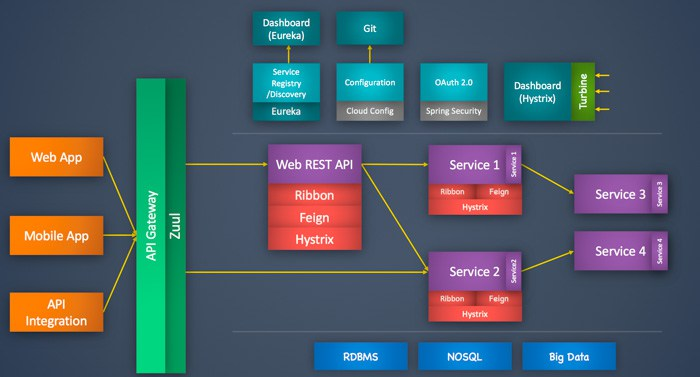
\includegraphics[scale=0.6, center]{images/netflix_microservices.jpg}
  \caption{Arquitectura de microservicios utilizando la tecnologia Netflix OSS. Tomado de \url{http://www.adeveloperdiary.com}}
  \label{fig:img3}
\end{figure}

Se utilizó la tecnologia Netflix OSS (Eureka, Feign, Zuul, Ribbon) para la arquitectura de microservicios ya que tiene una documentación bastante amplia y su uso es bajo licencia de código abierto, además se integra bastante bien con las herramientas con las que el equipo de desarrollo suele trabajar, las tecnologias utilizadas se listan a continuación:

\begin{itemize}
    \item Eureka: Herramienta para el descubrimiento de microservicios, es una consola de monitoreo donde se observan los microservicios de la plataforma, se configuró para que constantemente revise si un microservicio dejó de funcionar y automaticamente intente recuperarlo
    \item Zuul: Herramienta que hace las veces de Gateway (compuerta), el cual bajo una unica ip es capaz de direccionar una petición al microservicio apropiado.
    \item Feign: Herramienta para el nombramiento de servicios REST, facilita su creación y llamado
    \item Ribbon: Balanceador de carga en el caso de tener multiples replicas de la plataforma lo que mejora su tiempo de respuesta y solidez.
    \item MySQL: Motor de base de datos de código abierto, se utilizó gracias a su amplia documentación y conocimiento por parte de los desarrolladores
    \item Spring Boot: Framework que facilita la inyección de dependencias entre las capas de la arquitectura, es ampliamente recomendado en la documentacion de Netflix OSS
    \item Angular 5: Framework cuyo objetivo es aumentar las aplicaciones basadas en navegador con capacidad de Modelo Vista Controlador (MVC), su documentación y gran numero de funcionalidades hicieron que fuera seleccionado para el desarrollo.
\end{itemize}